\section{Diagrama de Casos de Uso}
\label{diag_casos}

\begin{center}
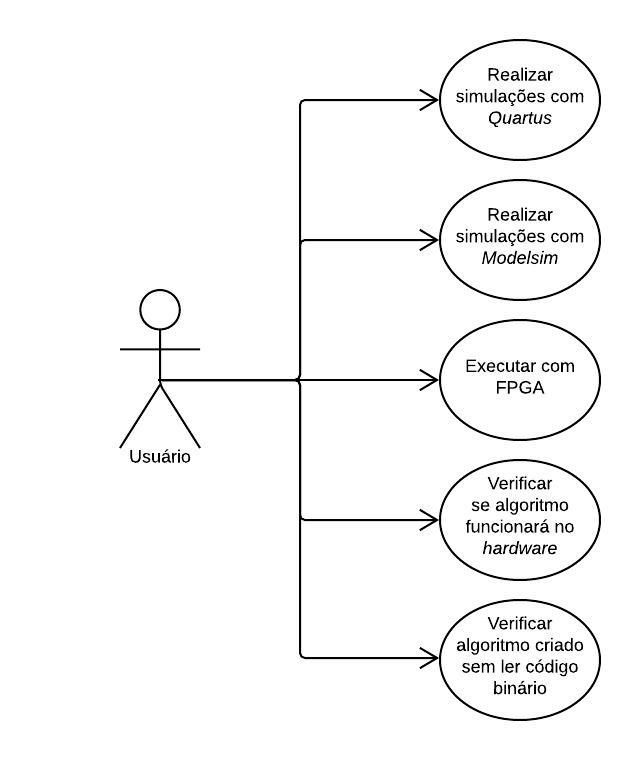
\includegraphics[scale=1]{apendice/images/diag_casos.jpeg}
\end{center}

\begin{description}
	\item[Realizar simula��es com \textit{Quartus}]: \textit{pyConv} gera o arquivo de inicializa��o de mem�ria para essa ferramenta (\textit{.mif});
	\item[Realizar simula��es com \textit{Modelsim}]: \textit{pyConv} gera o arquivo de inicializa��o de mem�ria para essa ferramenta (\textit{.mem}); 
	\item[Executar com FPGA]: \textit{pyConv} gera o arquivo de inicializa��o de mem�ria \textit{.mif} ap�s realizar simula��es para evitar erros;
	\item[Verificar se algoritmo funcionar� no \hw{}]: \textit{pyConv} realiza uma simula��o para verificar se o algoritmo inserido est� livre de problemas que leve a arquitetura a um estado de erro;
	\item[Verificar algoritmo criado sem ler c�digo bin�rio]: \textit{pyConv} gera um arquivo de texto com as instru��es e argumentos escritos conforme documenta��o da linguagem \py{}.
\end{description}

%\section{Diagrama de Sequ�ncia}
%\label{diag_seq}

%\begin{center}
%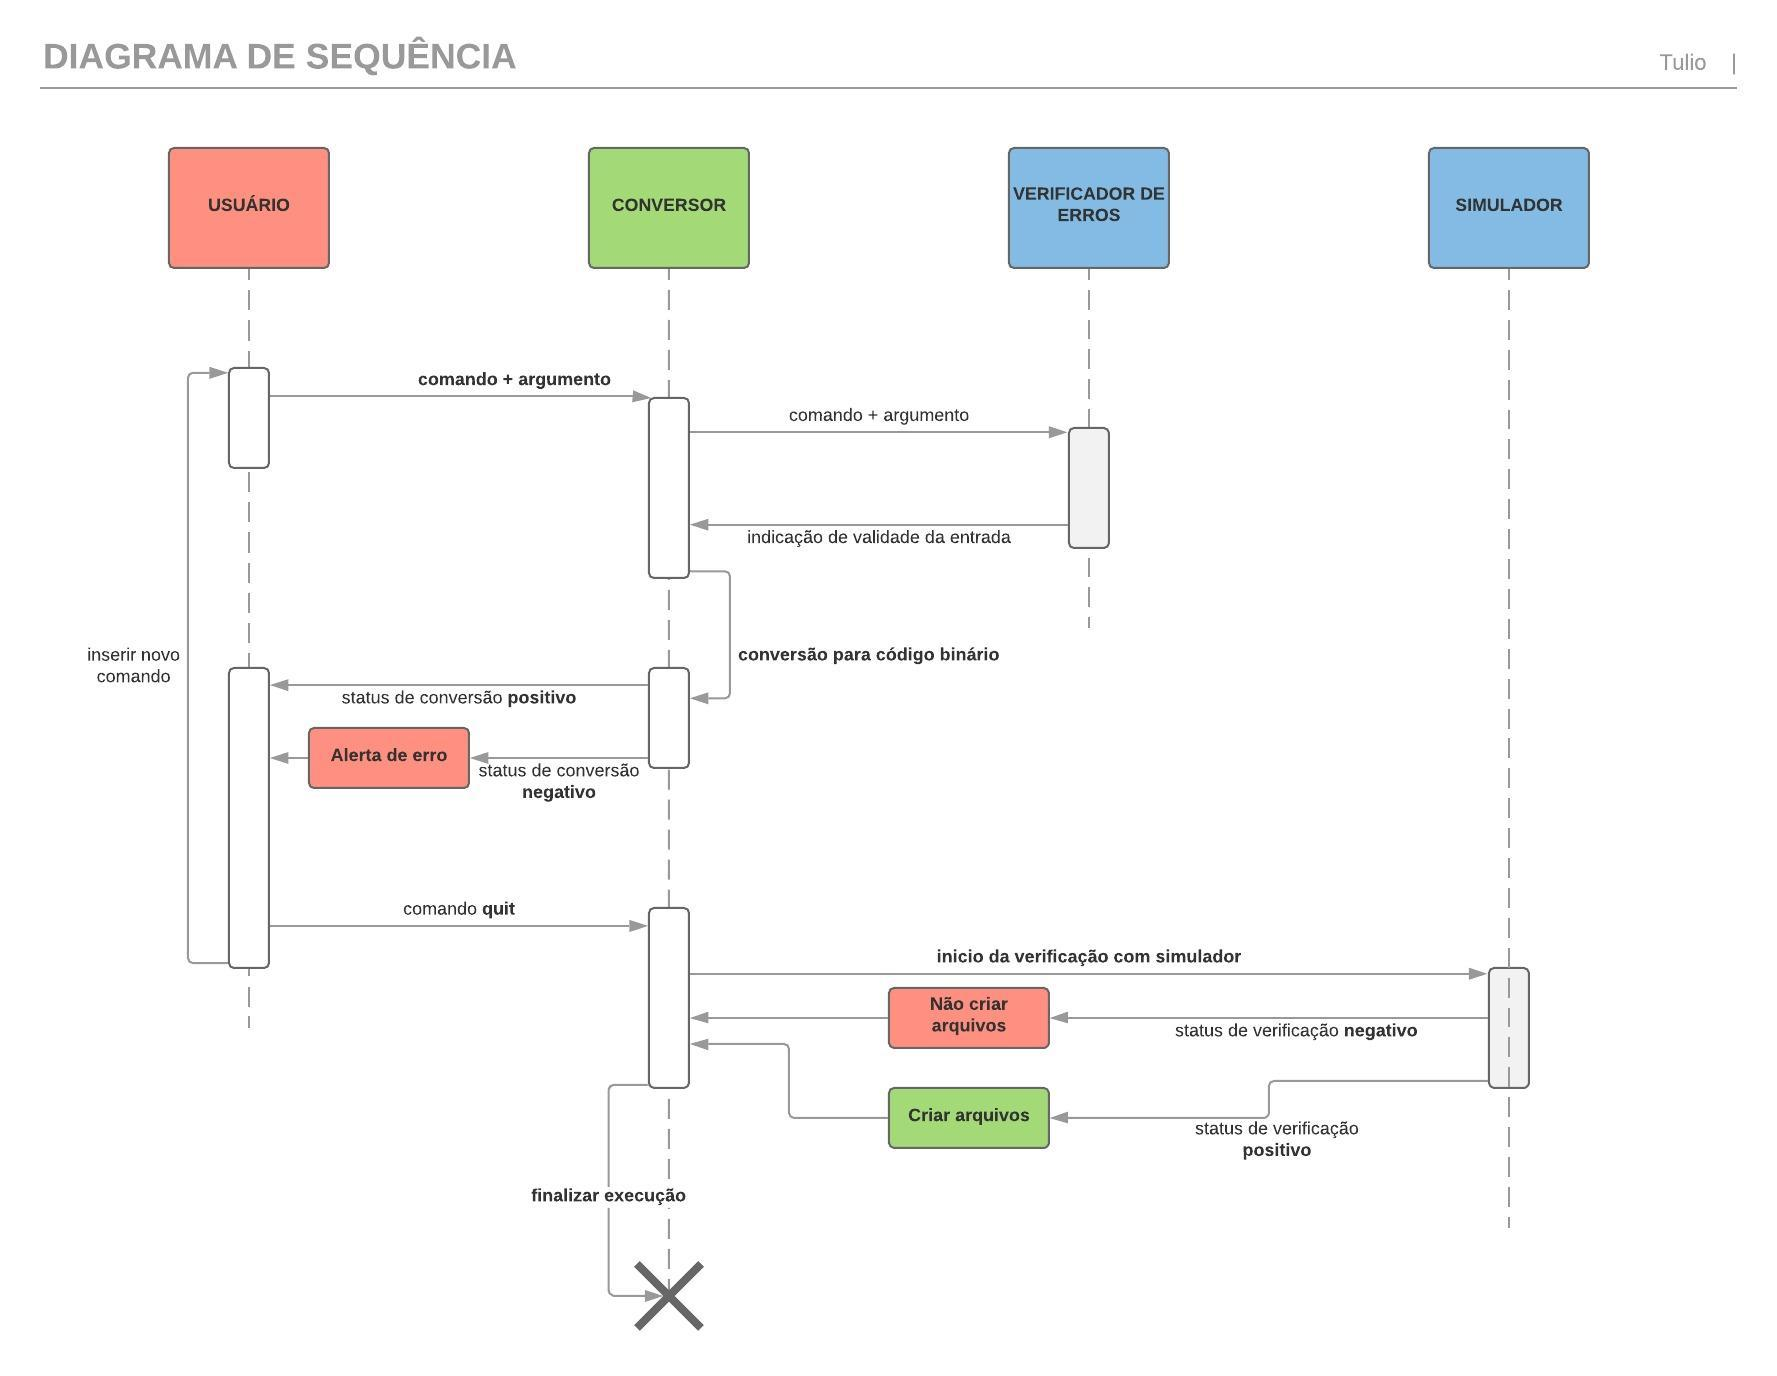
\includegraphics[scale=0.6]{apendice/images/diag_sequencia.jpeg}
%\end{center}

\section{Diagrama de Estados}
\label{diag_class}

\begin{center}
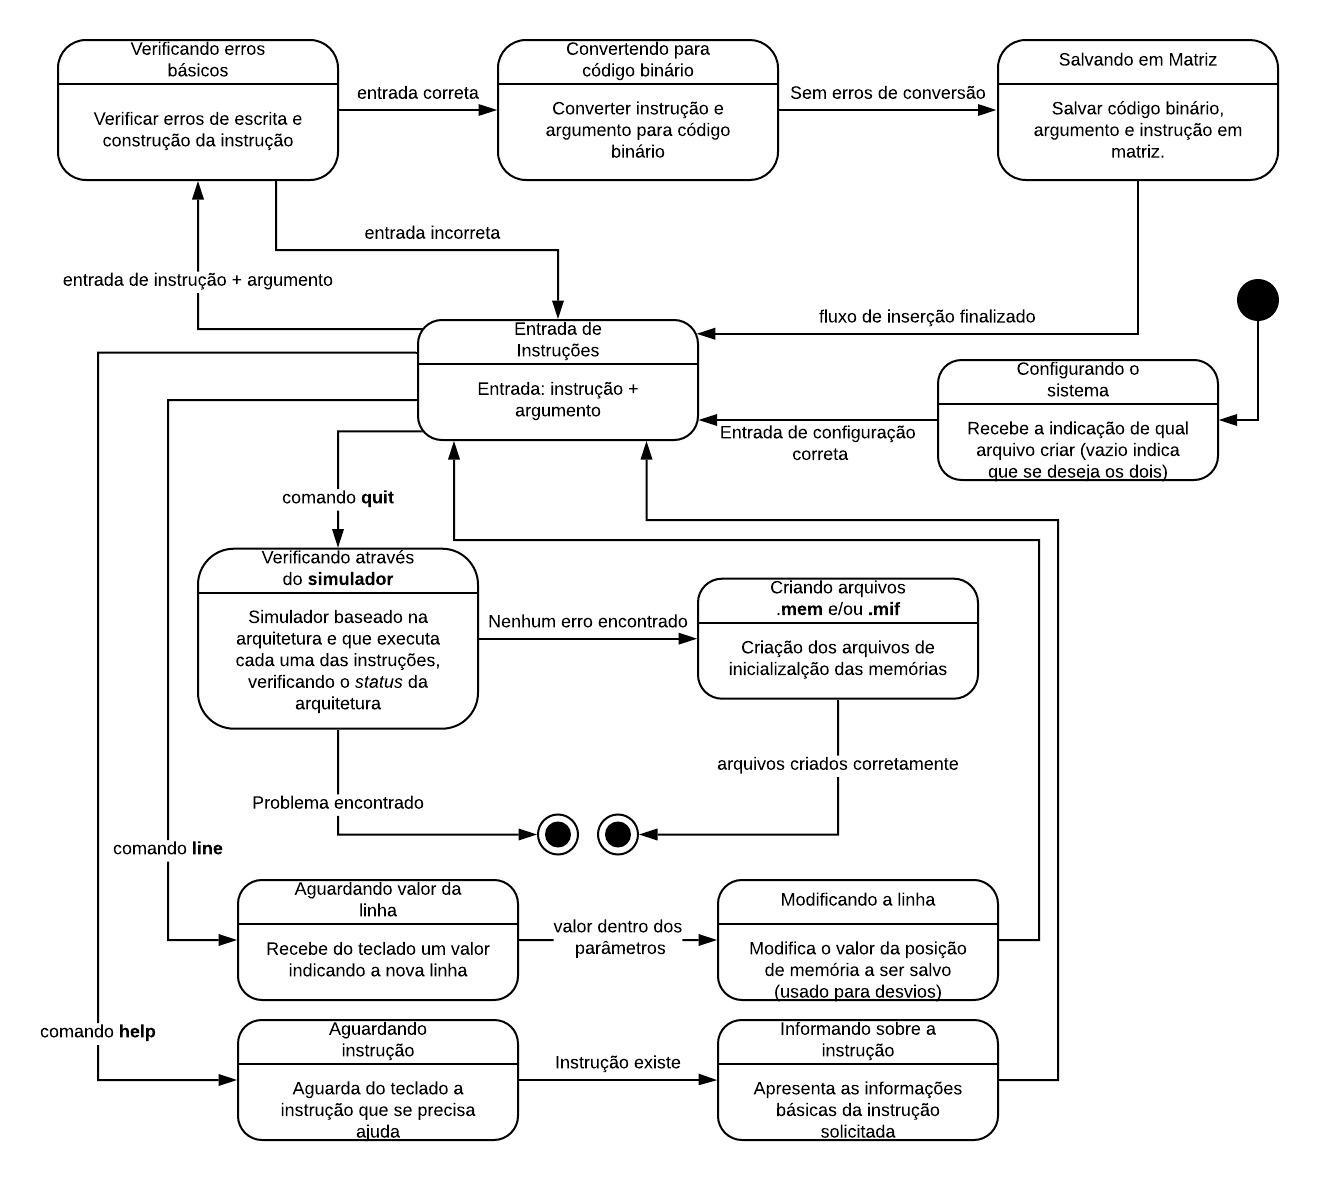
\includegraphics[scale=0.8]{apendice/images/diag_estados.jpeg}
\end{center}